\documentclass[tikz,border=10pt]{standalone}
\begin{document}
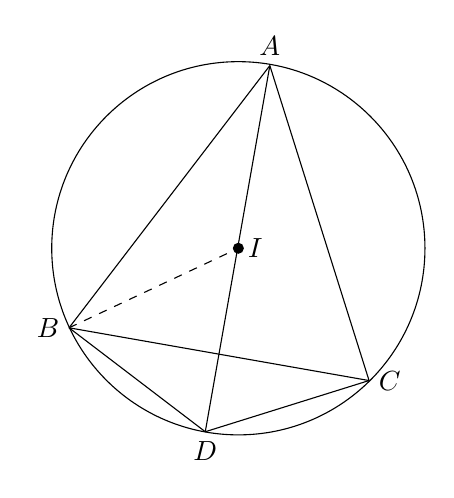
\begin{tikzpicture}
  % points
  \coordinate (A) at (0.40,2.32);
  \coordinate (B) at (-2.15,-1.01);
  \coordinate (C) at (1.66,-1.68);
  \coordinate (D) at (-0.42,-2.33);
  \coordinate (I) at (0,0);

  % circumcircle
  \draw (0,0) circle (2.37);

  % edges
  \draw (A) -- (B);
  \draw (A) -- (C);
  \draw (A) -- (D);
  \draw (B) -- (C);
  \draw (B) -- (D);
  \draw (D) -- (C);
  \draw[dashed] (B) -- (I);

  % point marker
  \fill (I) circle (2pt);

  % labels
  \node[above] at (A) {$A$};
  \node[left] at (B) {$B$};
  \node[right] at (C) {$C$};
  \node[below] at (D) {$D$};
  \node[right] at (I) {$I$};
\end{tikzpicture}
\end{document}
